\documentclass{article}
\usepackage{graphicx,fancyhdr,amsmath,amssymb,amsthm,subfig,url,hyperref}
\usepackage[margin=1in]{geometry}
\usepackage{xltxtra}
\usepackage{xgreek}
\usepackage{amsfonts}
\usepackage{amssymb}
\usepackage{amsmath}
\usepackage{amsthm}
\usepackage{mathtools}

\usepackage{caption}
\usepackage{ subfig}
\setmainfont[Mapping=tex-text]{Times New Roman}
%----------------------- Macros and Definitions --------------------------

%% FILL THIS OUT
\newcommand{\studentname}{Νικόλαος Ζαρίφης}
\newcommand{\suid}{03112178}
\newcommand{\exerciseset}{Exercise Set 1}
%% END



\renewcommand{\theenumi}{\bf \Alph{enumi}}

%\theoremstyle{plain}
%\newtheorem{theorem}{Theorem}
%\newtheorem{lemma}[theorem]{Lemma}

\fancypagestyle{plain}{}
\pagestyle{fancy}
\fancyhf{}
\fancyhead[RO,LE]{\bfseries\large NTUAthens}
\fancyhead[LO,RE]{\bfseries\large Θεωρία γράφων}
\fancyfoot[LO,RE]{\bfseries\large \studentname: nick.zarifis@hotmail.com}
\fancyfoot[RO,LE]{\bfseries\thepage}
\renewcommand{\headrulewidth}{1pt}
\renewcommand{\footrulewidth}{1pt}

\graphicspath{{figures/}}
\usepackage{tikz}
%-------------------------------- Title ----------------------------------

\title{Θεωρία γράφων \\ \exerciseset}
\author{\studentname \qquad  ID: \suid}

%--------------------------------- Text ----------------------------------
\DeclarePairedDelimiter\floor{\lfloor}{\rfloor}
\newtheorem{lemma}{Lemma}
\begin{document}
\maketitle

\section*{Άσκηση 1}
\begin{tikzpicture}
\tikzstyle{main node}=[circle,fill=black!28,minimum size=17pt,inner sep=2pt]
	\node[main node] (1) {A};
	\node[main node] (2) [below left of=1] {B};
	\node[main node] (3) [right of=2] {C};

\end{tikzpicture} \\
Ο γράφος μας θα έχει το παραπάνω σχήμα.Αν λοιπόν ισχύει $ B+C\ge \frac{2n}{3}$ τότε κάθε ακμή στον Α θα έχει βαθμό δ(Α)$ \ge \frac{2n}{3}$.Αλλιώς θα έχουμε: $ B+C< \frac{2n}{3} \rightarrow A > \frac{n}{3}$. Χωρίς βλάβη της γενικότητας έστω ότι οι κόμβοι του C$<\frac{n}{3}$ Τότε όμως 
αναγώμαστε στην πρώτη περίπτωση , όμοιος για για C$>\frac{n}{3}$ με την διαφορά ότι τώρα γίνεται για την κορυφή Β. 
\section*{Problem 2}
\begin{enumerate}
\item[1]
(4,4,3,2,1) Δεν είναι γραφική ακολουθία γιατί έχουμε 2 κορυφές που συνδέονται με όλες τις κορυφές ενώ η τελευταία συνδέεται μόνο με μια.
\item[2]
(4,3,2,1) Η ακολουθία δεν είναι γραφική γιατί έχουμε 4εις κορυφές και μια κορυφή με βαθμό 4.
\item[3]
(7,7,6,5,4,4,3,2) $\rightarrow $ (6,5,4,3,3,2,1) $\rightarrow $ (4,3,2,2,1,0) $\rightarrow$ (2,1,1,0,0) \ η οποία είναι γραφική. Χρησιμοποιώντας την γνώστη μέθοδο αποδείξεις του αντιστρόφου του θεωρήματος Havel-Hakimi, έχουμε τον ακόλουθο γράφο.\footnote{Χρησιμοποιήσα το One-click Layout}\\ 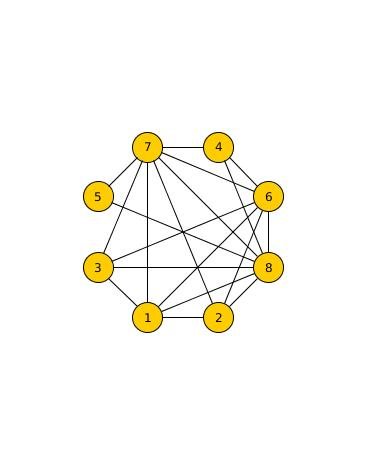
\includegraphics[height=200pt,width=150pt]{ex2prob3} 
\item[4]
(7,6,6,5,4,3,2,1) $\rightarrow$ (5,5,4,3,2,1,0) δεν είναι γραφική για τον ίδιο λόγο με την [1] .
\item[5]
(7,4,3,3,2,2,2,1,1,1) $\rightarrow$ (3,2,2,1,1,1,0,1,1) $\rightarrow$ (3,2,2,1,1,1,1,1,0) $\rightarrow$ (1,1,0,1,1,1,1,0) $\rightarrow$ (1,1,1,1,1,1,0,0) που είναι γραφική άρα ο γράφος θα είναι: \\ 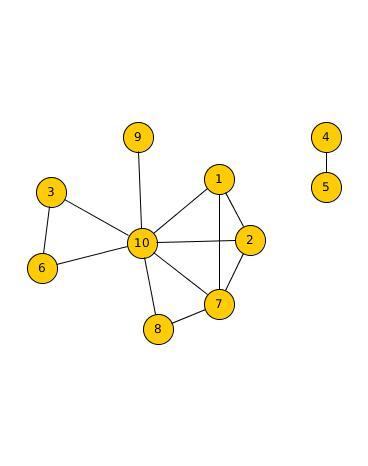
\includegraphics[height=200pt,width=150pt]{ex2prob5} 
\item[6]
(5,5,3,2,1,x) δεν είναι γραφική λόγο της κορυφής βαθμού 1, που πρέπει να συνδεθεί τουλάχιστον με 2 κορυφές όπως η [1]
\end{enumerate}
\section*{Problem 3}
\begin{enumerate}
\item[iα]Γνωρίζουμε ότι ένα γράφημα είναι διμερές ανν έχει κύκλους μόνο άρτιου μεγέθους. Μπορούμε να σκεφτούμε ένα πλέγμα σαν ένα τυχαίο περίπατο,που πάμε είτε δεξιά είτε αριστερά, πάνω κι κάτω. Ορίζω συνάρτηση τω:\[
\mbox{f}(x)=\left\{
\begin{array}{rl}
1 & \mbox{if left} \\
0 & \mbox{otherwise} \\
-1 & \mbox{if right}
\end{array} \right.
\] 
\[
\mbox{g}(x)=\left\{
\begin{array}{rl}
1 & \mbox{if up} \\
0 & \mbox{otherwise} \\
-1 & \mbox{if down}
\end{array} \right.
\] 
Όπως βλέπουμε για να έχω κύκλο πρέπει το $\sum_{i\in Moves} f(x_i)=0$ Και $\sum_{i\in Moves} g(x_i)=0$ το οποίο συμβαίνει μόνο όταν έχουμε ίδιο πλήθος $1$,$-1$ άρα έχουμε άρτιες κινήσεις, άρα διμερές γράφημα. Άλλη προσσεγγιση θα είχα αν απλά απο κάθε κορυφή βάζαμε σε διαφορετικό σύνολο την γειτονιά της, τότε θα έφτιαχνα ένα διμερές γράφημα.
\item[ib] προφανές ο ελάχιστον κύκλος είναι ο $C_4$. Για να βρούμε τον μέγιστο κύκλο θα πρέπει να υπάρχουν 2 ακμές σε κάθε κόμβο που θα μείνουν.Σίγουρα θα είναι παραπάνω από το 2p+2q μιας κι μπορούμε να αφήσουμε ένα περίγραμμα αλλά βλέπουμε πως δημιουργώντας ένα πέταλο μπορούμε να μεγαλώσουμε κι άλλο το φράγμα.
\item[iiα]
Ικανή κι αναγκαία συνθήκη είναι κι τα δύο γραφήματα να μην έχουν καμία ακμή. Αυτό συμβαίνει γιατί αν έχει έστω κι μία τότε αφού όλες οι κορυφές ενόνται με όλες τις ακμές του άλλου γράφου φαίνεται ότι οι κορυφές του κάθε γράφου πρέπει να είναι σε διαφορετικά σύνολα, όμως αν υπάρχει μια ακμή τότε θα είχαμε 2 κορυφές στο ίδιο σύνολο που θα είχαν ακμή άρα δεν θα ήταν διμερές.Το αντίστροφο φαίνεται αμέσως,γιατί μετά την σύνδεση θα έχω το $K_{|V(G)|,|V(H)|}$.
\item[iiβ]
Εδώ πέρα έχουμε ως ικανή κι αναγκαία συνθήκη τα γραφήματα να είναι διμερές. Γιατί αν το ένα δεν είναι τότε αφού δεν αφαιρείται καμιά ακμή θα μπορώ να βρω έναν κύκλο περιττού μήκους κι να υπάρχει κι στο γινωμένο αυτός.Αντίστροφα αν είναι διμερές τότε επειδή ισχυεί το γινόμενο κι η επιμεριστική, μπορούμε να το σπάσουμε το κάθε γραφο σε 2 σύνολα που δεν έχουν ακμές μεταξύ τους. $A=A_1 \cup A_2$ και $B=B_1 \cup B_2$ Έτσι το γίνομενο θα είναι τις μορφής :$A_i X B_j$ χωρίζοντας σε σύνολα έτσι ωστε να έχουμε μαζί ότι δεν έχουν ακμές μεταξύ τους βλέπουμε ότι τελικά είναι πάλι διμερές.
\end{enumerate}
\section*{Problem 4}
Γενικά ισχύει ότι $\Delta(G) \ge \delta(G)$ .Αφού δεν είναι κανονικό δεν υπάρχει ισότητα άρα ας υποθέσουμε ότι $\Delta(G) = \delta(G)+1$. Από λήμμα χειραψίας έχουμε $rn=\sum_{i \in I_1}\Delta(G) + \sum_{i \in I_2}\delta(G)$ όπου το $|I_1|=k $ αθροίζει σε όσες έχουν βαθμό μέγιστο κι το $I_2$ στις υπόλοιπες αντίστοιχα.Άρα $rn=k+n\delta(G)\rightarrow n(r-\delta(G))=k$ το όποιο σύμφωνα με τις ανισοσεις έχει λύση μόνο για $k=n $ πράγμα άτοπο γιατί δεν είναι κανονικό άρα: $\Delta(G) \ge \delta(G)+2$
\section*{Problem 5}
Βλέποντας την απόδειξη θα πρέπει πρώτα να κατασκευάσουμε το σύνολο $\{2,3,4\}$ κι μετά το σύνολο $\{3,5,6,7,9\}$ κι στο τέλος έχω προσθέσει ένα realocation.
\begin{figure}[ht!]
	\centering
	\subfloat[$\{2,3,4\}$ ]{{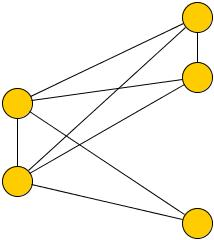
\includegraphics[height=150pt,width=150pt]{ex51}}
	}
	\qquad
	\subfloat[$\{3,5,6,7,9\}$]{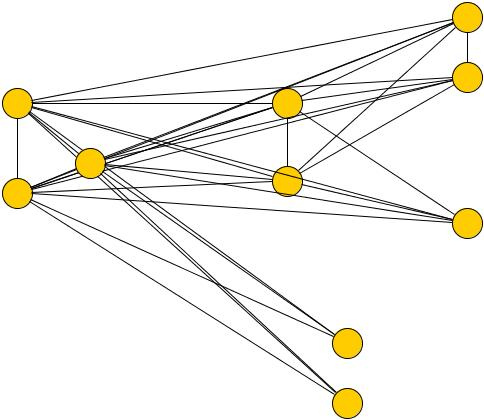
\includegraphics[height=150pt,width=120pt]{ex52}}
	\qquad
	\subfloat[relocate]{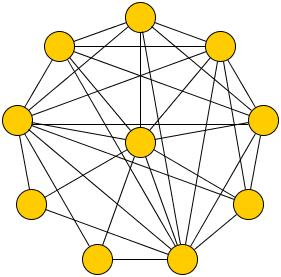
\includegraphics[height=150pt,width=120pt]{ex5relocate}}\caption{graphs}
	
	
\end{figure}
\section*{Problem 6}
 Ξέρουμε ότι τουλάχιστον μια θα συνδέεται με τουλάχιστον τις μισές κι μια ακόμα. (Δεν μας ενδιαφέρει να δείξουμε κανένα απο τα 2 για παραπάνω.)
	Θα πρέπει να βάλουμε όσες περισότερες ακμές γίνεται αυτό γίνεται βάζοντας στο ίδιο σύνολο τις ν/2 +1 ακμές (δεν πρέπει να συνδέονται γιατι θα εχουμε τριγονο), ο μόνος τρόπος για να βάλουμε περισότερες ακμές είναι να δημιουργήσουμε έναν πλήρες δημερές γράφο ωστε να μην σχηματίζεται τρίγονο γιατί αν στο άλλο σύνολο συνδέονται 2 κορυφές τότε δεν μπορούν να συνδεθουν κι οι 2 αυτές με μια απο το άλλο σύνολο κι έτσι για να βγεί ο αριθμος των ακμών θα έχουμε τριγονο. Τέλος επειδή το δημέρες θα έχει $\floor{n^2/4}$ ακμές κι έχουμε παραπάνω σίγουρα θα έχουμε τρίγονο.  
\begin{proof}
Θα το δείξω με επαγωγή με βήμα 2 ότι το φράγμα είναι το καλύτερο.. Έχουμε ότι $\floor {\frac{(n+2)^2}{4}} = n+1 +\floor {\frac{n^2}{4}} $. Έχω λοιπόν ένα γράφημα με n κορυφές κι δεν έχει μέσα το $K_3$.Αυτό σημαίνει πως μπορώ να κάνω την ακόλουθη κατασκευή. Ξεκινάω από μια ακμή κι ότι απέχει από αυτή ζυγή απόσταση πάει στον πρώτο κόμβο κι οι υπόλοιπες στον δεύτερο κόμβο, κι ενώνω τους 2 κόμβους.Σύνολο n+1 ακμές.Δεν υπάρχει τρίγωνο γιατί : προφανές γιαυτό που απέχουν μεταξύ τους 2 απόσταση, τώρα γιαυτό που είναι διαδοχικά έχουμε συνολική απόσταση 4 άρα δεν έχει κύκλο μήκους 3. για n=1,2 είναι τετριμμένο άρα από μαθηματική επαγωγή έχω για κάθε n,
\end{proof}
Με λίγο ψάξιμο βρίσκουμε ότι η παραπάνω άσκηση θα μπορούσε να λυθεί άμεσα από το θεώρημα του Turan.
\section*{Problem 7}
Ας το γενικεύσουμε:\\ \textbf{Υπάρχει 3-κανονικό γράφημα με $|V|>3$ κορυφές που να περιεχέι τουλάχιστον μια φορά το $C_k$ για $3\le k\le |V|$} 
\begin{proof}
	Για $|V|=4$ έχουμε το 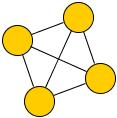
\includegraphics[height=50pt,width=50pt]{ex7}.\\
	Έστω G  γράφος με n κορυφές. Για να πάμε στο βήμα $n+1$ πρέπει να προσθέσουμε μια κορυφή κι να δημιουργήσουμε έναν κύκλο με μήκος κατά ένα μεγαλύτερο απο τον προηγούμενο μέγιστο. Αυτό γίνεται εύκολα , παίρνουμε τον μέγιστο κύκλο κι σε δύο διαδοχικούς του κόμβους ενώνουμε 2 ακμές από τον νέο μας κόμβο. Έτσι προσθέσαμε έναν κύκλο κατά ένα μεγαλύτερο.Άρα αποδείξαμε έναν τρόπο κατασκευής του.Την άλλη ακμή την βάζουμε όπου θέλουμε μιας κι δεν επηρεάζει το αποτέλεσμα.
	\end{proof}
Έστω ότι έχει μόνο ένα κύκλο για κάθε k ως το 10. Αυτό σημαίνει πως αν αφαιρέσουμε ακμές θα έχουμε έναν τον $C_{10}$.Για να σχεδιάσουμε όμως τον κύκλο μήκους 6 θα πρέπει να χωρίσουμε τον κύκλο σε δύο κομμάτια αυτό σημαίνει ότι αν πάρεις την άλλη διαδρομή θα έχεις έναν δεύτερο κύκλο μήκους 6 άρα δεν γίνεται. 
\section*{Problem 8}
$\leftarrow$ \\
Εύκολα φαίνεται αν προσθέσουμε την κορυφή στον πρώτο σύνολο κι την ενώσουμε με αυτές από το δεύτερο σύνολο που μειώθηκε κατά ένα ο βαθμός.\\
$\ \  \ \ \ \ \rightarrow$\\
Παρόμοια με την απόδειξη με τις γραφικές κι άνηγμένες γραφικές έχουμε ότι: Αν συνδέετε διαδοχικά με τις πρώτες έχουμε το αποτέλεσμα αλλιώς: 
$\exists v_k,v_j \in V_2$ ώστε $(v_1,v_k)\in E$ και  $(v_1,v_j)\notin E$με βαθμό η δεύτερη μεγαλύτερο από την πρώτη άρα $\exists v_l \in V_1$ ώστε $(v_l,v_j)\in E$ και  $(v_l,v_k)\notin E$.Τότε χρησιμοποιούμε μεταγωγή ανάμεσα σε αυτές τις κορυφές. Κι έτσι η $v_1$ συνδέεται με κορυφές μεγαλύτερου βαθμού από πριν, κάνοντας την διαδικασία συνέχεια φτάνουμε στο αποτέλεσμα.
\section*{Problem 9}
\begin{lemma}
Αν ο $G\sim\bar{G}$ τότε $\forall v\in V(G), \exists x\in V(G):d(v)+d(x)=n-1 $
\end{lemma}
\begin{proof}
	Έστω $v\in V(G):d(v,G)=k$\footnote{πρώτο όρισμα: κορυφή,δεύτερο: γράφος που ανήκει} τότε $d(v,\bar{G})=n-k-1$ από ορισμό συμπληρωματικού γράφου.Όμως αφού $G\sim \bar{G}\Rightarrow \exists u\in V(\bar{G}):d(u)=k$ \footnote{αλλιώς δεν θα μπορούσαν να είναι ισομορφικά} άρα $d(v,\bar{G})+d(u,\bar{G})=n-1$ κι $d(v,G)+d(u,G)=n-1$
\end{proof}
\begin{enumerate}
\item[1]
Ξαίρουμε ότι οι $G_1,G_2$ είναι αυτοσυμπληρωματικοί . Αφού έχουμε ενώσει όλες τις ακμές  με βαθμό $< \frac{n_2}{2}$ του $G_2$ με όλες τις κορυφές του $G_1$ αν τότε οι υπόλοιπες ακμές του $G_2$ ενωθούν με όλες του $G_1$ στον συμπληρωματικό τότε θα είναι αυτοσυμπληρωματικός.Από το προηγούμενο λήμμα υπάρχουν ακριβώς το ίδιο πλήθος κορυφών με βαθμό  $\ge \frac{n_2}{2}$ άρα τελικά θα είναι αυτοσυμπληρωματικός. Άμα ήταν περιττός ο αριθμός των κορυφών δεν θα ίσχυε γιατί τότε θα είχαμε 2 κορυφές με ίδιο βαθμό όπου θα ήταν οι κορυφές του λήμματος κι έτσι δεν θα είχαμε αυτοσυμπληρωματικό γράφημα .
\item[2]
Θα το κατασκευάσουμε επαγωγικά. Για $n=1$ έχουμε το $C_5$.Έστω ότι έχουμε το γράφημα για $n=5^k$ αν λοιπόν πάρουμε 5 φορές αυτό το γράφημα κι ενώσουμε το κάθε γράφημα με τα άλλα έτσι ώστε αν το κάθε ένα ήταν μια κορυφή θα δημιουργούσαν το $C_5$, η ένωση γίνεται ενώνοντας όλες τις κορυφές με όλες τις ακμές. Το νέο γράφημα είναι κανονικό γιατί όλες οι κορυφές έχουν βαθμό$d(G_i)=d(G_{i_prev}+2*5^k)$ , και είναι ισομορφικό γιατί αν θεωρήσουμε το κάθε γράφο ως μια κορυφή κάνει το  $C_5$. \footnote{Ο τρόπος με τον όποιο δημιουργήσαμε τον γράφο μας επιτρέπει να τα θεωρήσουμε ως κορυφές.}. Άρα από επαγωγή έχουμε το αποτέλεσμα.
\item[3]
Ομοίως εδώ επαγωγικά.\\ 
$\bullet$\ Για $n=4k$. Για κ=1 έχουμε το $P_4$. Έστω για n=4k πάμε στο $n=4k+4 $ φέρνοντας ένα $P_4$. Όμως το $P_4$ μπορεί να θεωρηθεί ως ο $G_2$ του ερωτήματος 1. Άρα έτσι δημιουργούμε ένα αυτοσυμπληρωματικό γράφημα. Έτσι απο επαγωγική υπόθεση για κάθε $k$ έχουμε γράφημα.
\\ $\bullet$\ Ομοίως με παραπάνω.Για $n=4k+1$.\footnote{$k=1$ τετριμμένο}  Για κ=1 έχουμε το $C_5$. Έστω για n=4k+1 πάμε στο $n=4k+5 $ φέρνοντας ένα $P_4$. Όμως το $P_4$ μπορεί να θεωρηθεί ως ο $G_2$ του ερωτήματος 1. Άρα έτσι δημιουργούμε ένα αυτοσυμπληρωματικό γράφημα. Έτσι από επαγωγική υπόθεση για κάθε $k$ έχουμε γράφημα. 
\end{enumerate}
\section*{Problem 10}
\begin{enumerate}
\item[1]
Θα κατασκευάσω επαγωγικά ένα τέτοιο γράφημα. Όταν έχω μια κορυφή δεν έχω καμία ακμή. Έπειτα σε κάθε βήμα προσθέτω μια κορυφή κι την ενώνω με ακμή που φεύγει από αυτή με όλες τις άλλες μέχρι να έχω ν κορυφές.Για $P(1)$ ισχύει, έστω $P(n)$, έπειτα παίρνω μία κορυφή κι την ενώνω με όλες τις άλλες . Όμως από υπόθεση όλες οι προηγούμενες είχαν διαφορετικό in-degree άλλα πάλι θα έχουν γιατί αυξήθηκαν όλοι κατά ένα.Όπως επίσης μόνο η τελευταία κορυφή θα έχει out-degree $n$. Άρα από επαγωγή ισχύει. 
\item[2]
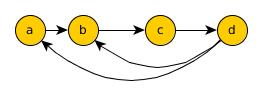
\includegraphics[height=100pt,width=100pt]{ex10prob2} \\
Έστω ότι υπάρχει μια κορυφή με ελάχιστη απόσταση 3 (για να υπάρχει μεγαλύτερη απόσταση πρέπει να υπάρχει κι μια με 3), όπως στο σχήμα, τότε ο μόνος τρόπος να ισχύει είναι να υπάρχουν οι ακμές με αυτή την μορφή. Όμως αν κάνουμε την κορυφή με απόσταση 3 βασιλιά τότε θα απέχει 0 από την πρώτη κι 2 με όσες άπεχε η πρώτη με 1 και με όσες άπεχε 2 η κορυφή 0 θα απέχουν είτε 2 είτε ένα κι έχει παραπάνω κορυφές πιο κοντά(απόσταση 1 ή 2) από ότι η προηγούμενη. Κάνοντας την ίδια διαδικασία συνέχεια βρίσκουμε μια κορυφή βασιλιά στο πολύ n-1 βήματα.
\item[3]
\begin{figure}[ht!]
	\centering
	\subfloat[k=5] {{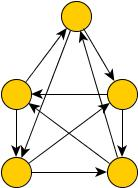
\includegraphics[height=50pt,width=50pt]{ex105}}
	}

	\qquad
	\subfloat[k=6]{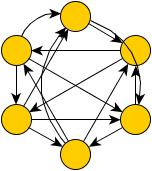
\includegraphics[height=70pt,width=80pt]{ex106}}\caption{graphs}
	
\end{figure} 
Θα χρησιμοποιήσω επαγωγή. Στα παραπάνω σχήματα κατασκεύασα γράφους με όλες τις κορυφές βασιλιάδες για k=5,6. Τώρα θα χρησιμοποιήσω επαγωγή με βήμα 2. Έστω ότι έχω τον γράφο για k=n. Προσθέτω δυο κόμβους έτσι ώστε στον πρώτο κόμβο ενώ τις n κορυφές με κατεύθυνση προς τον κόμβο. Και φέρνω μια ακμή απο τον πρώτο κόμβο προς τον δεύτερο κόμβο ,τέλος ενώνω όλες τον δεύτερο κόμβο με ακμή προς όλες τις κορυφές του γράφου.
Τώρα κάθε κορυφή είναι βασιλείας γιατί: όλες η κορυφές πάνε στην πρώτη κορυφή με ένα βήμα κι στην δεύτερη με 2. Η πρώτη κορυφή πάει στην δευτερή με ένα βήμα κι σε όλες τις άλλες με 2. Κι τέλος η δεύτερη κορυφή πάει σε όλες με κατεύθυνση με 1 βήμα κι στην πρώτη πάει με 2 βήματα(ένα βήμα προς οποιαδήποτε άλλη κι άλλο ένα από αυτή στην πρώτη.).Άρα έχω δείξει πως από $P(k)\rightarrow P(k+2)$ και αφού έχω απόδηξει για k=5,6 έχω ότι για κάθε $n>4$ υπάρχει τέτοιος γράφος  .
\end{enumerate}
\end{document}
